\section{实验结果与分析}
经过综合实现,我们可以在开发板上看到测试的结果。我们分以下几个部分验证实验结果的正确性
\subsection{异常与中断跳转}
当触发异常或中断时,清空尚未结束的所有指令,并跳转至中断/异常处理程序\\
遇到ecall指令触发异常
\begin{figure}[H] %H为当前位置,!htb为忽略美学标准,htbp为浮动图形
	\centering %图片居中
	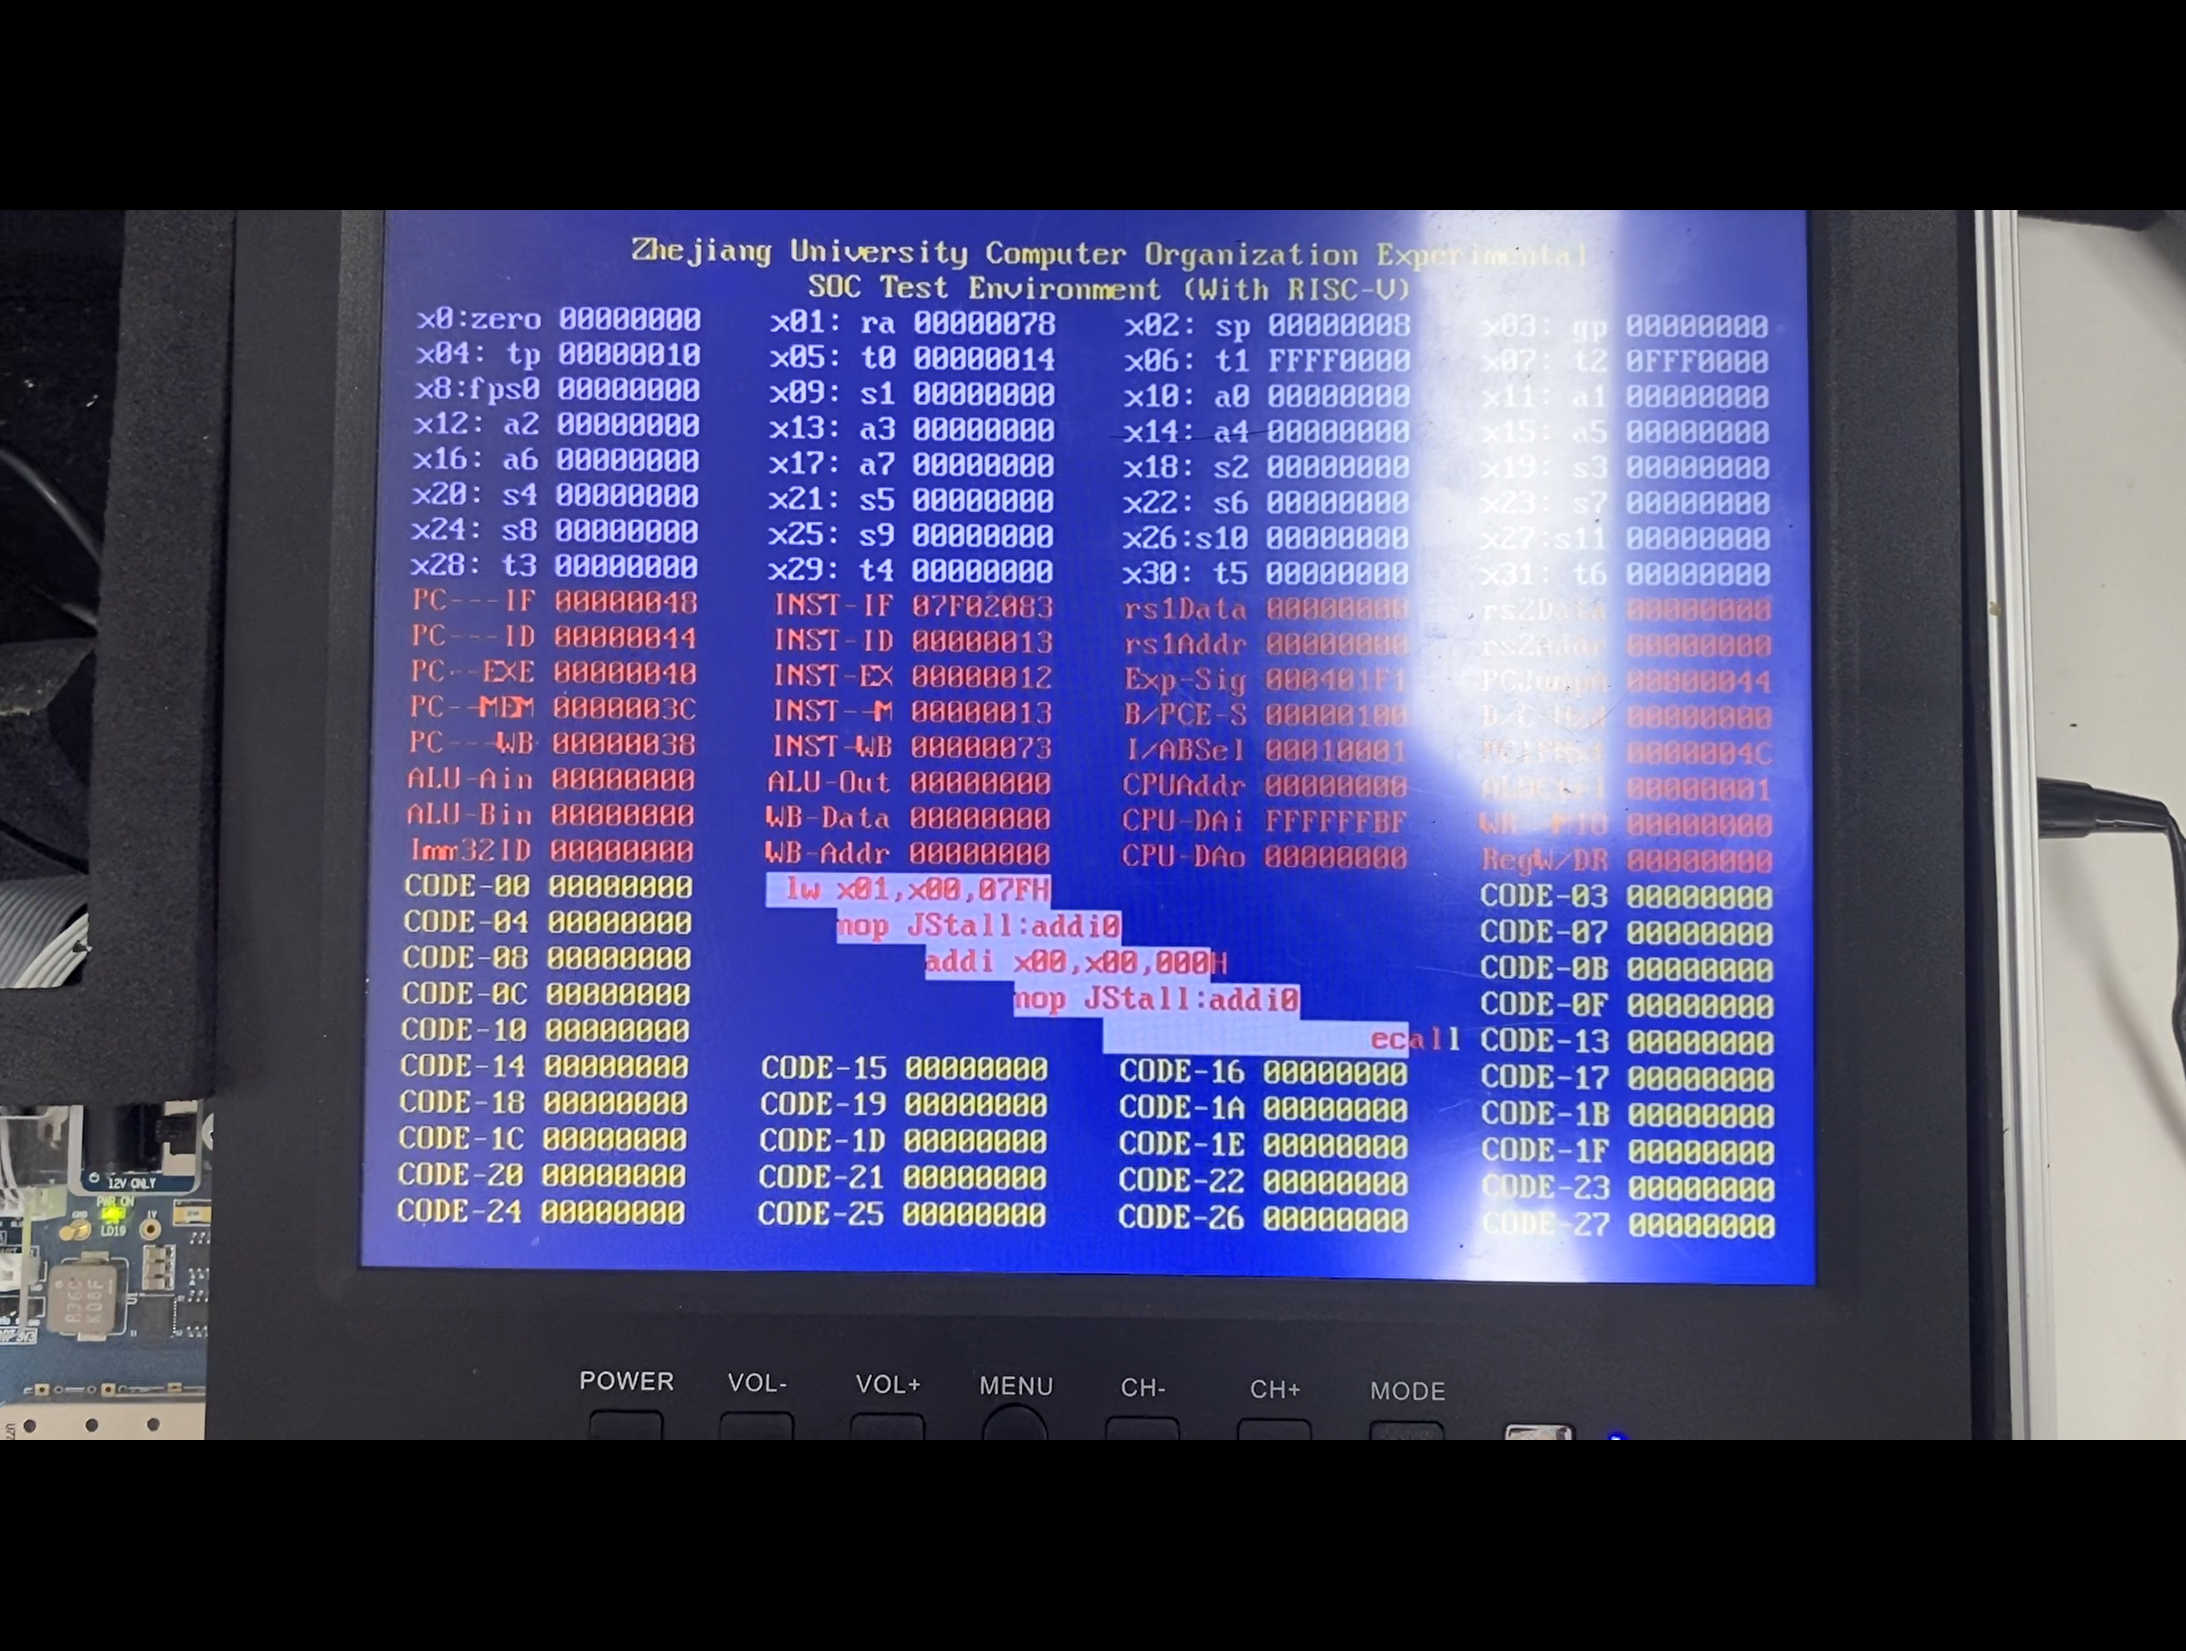
\includegraphics[width=1.0\textwidth]{figs/7.png} %插入图片,[]中设置图片大小,{}中是图片文件名
	\caption{验证结果图1} %最终文档中希望显示的图片标题
	\label{Fig.19} %用于文内引用的标签
\end{figure}
进入trap时清空先前指令
\begin{figure}[H] %H为当前位置,!htb为忽略美学标准,htbp为浮动图形
	\centering %图片居中
	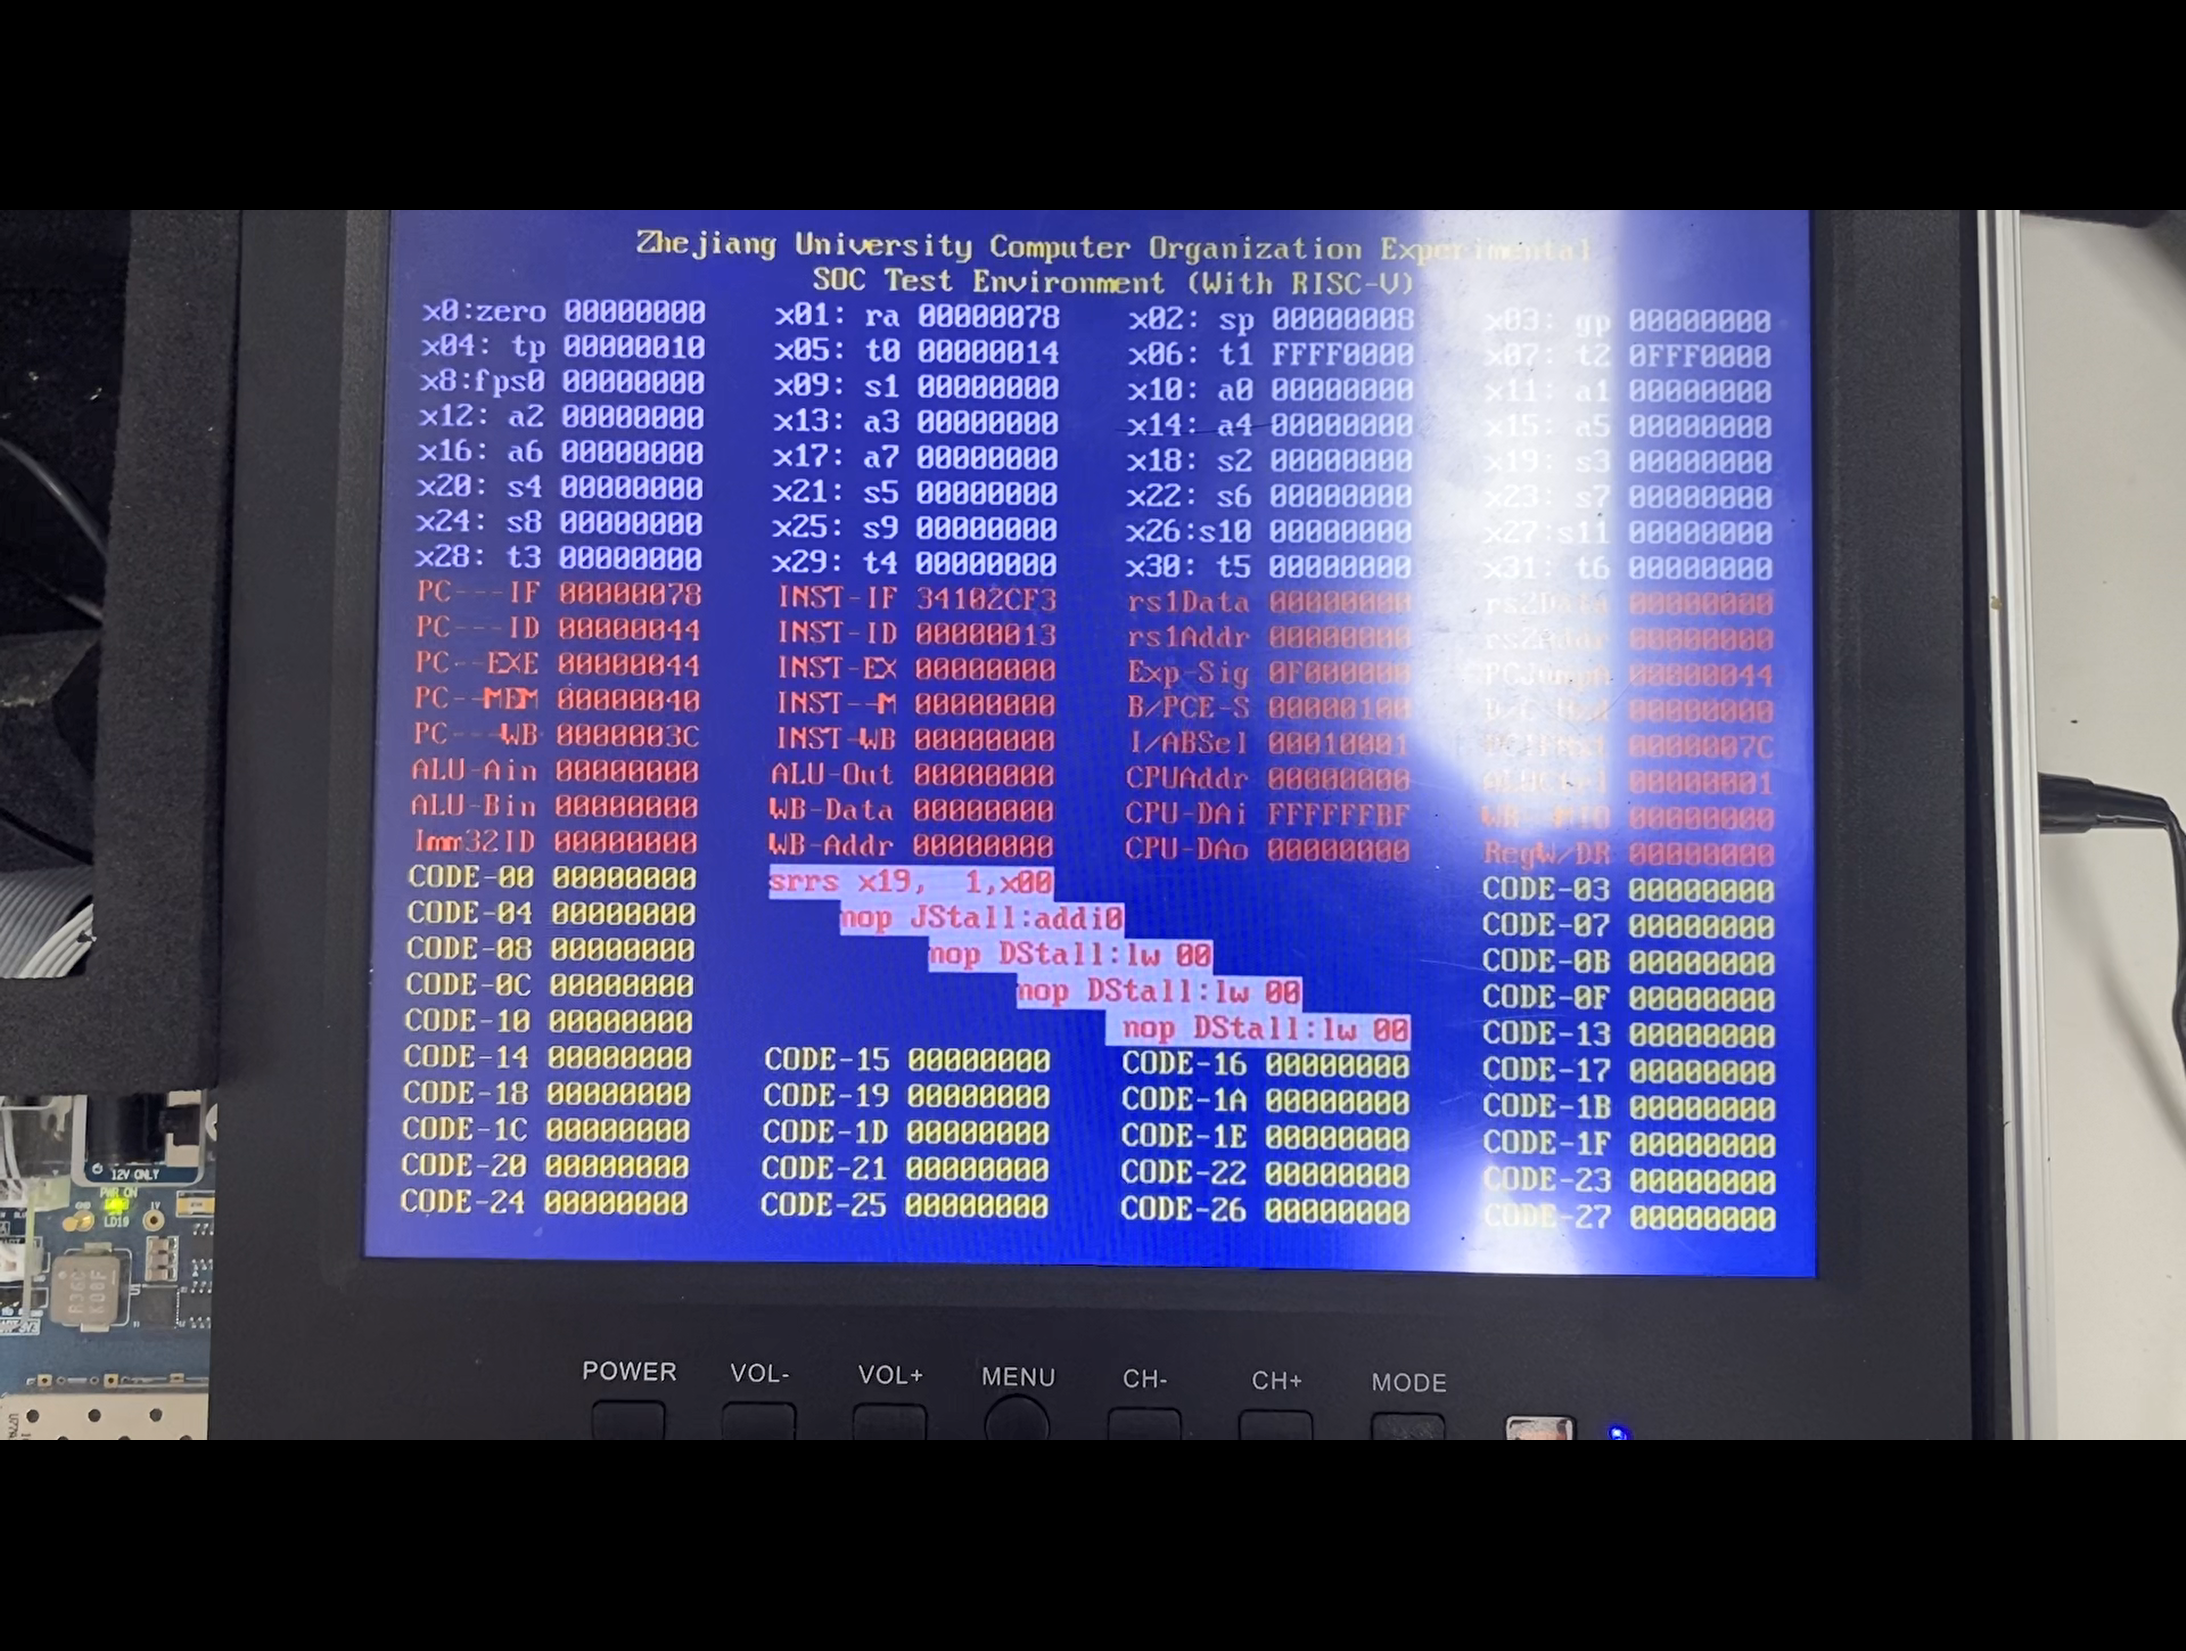
\includegraphics[width=1.0\textwidth]{figs/8.png} %插入图片,[]中设置图片大小,{}中是图片文件名
	\caption{验证结果图2} %最终文档中希望显示的图片标题
	\label{Fig.20} %用于文内引用的标签
\end{figure}
trap中指令的运行
\begin{figure}[H] %H为当前位置,!htb为忽略美学标准,htbp为浮动图形
	\centering %图片居中
	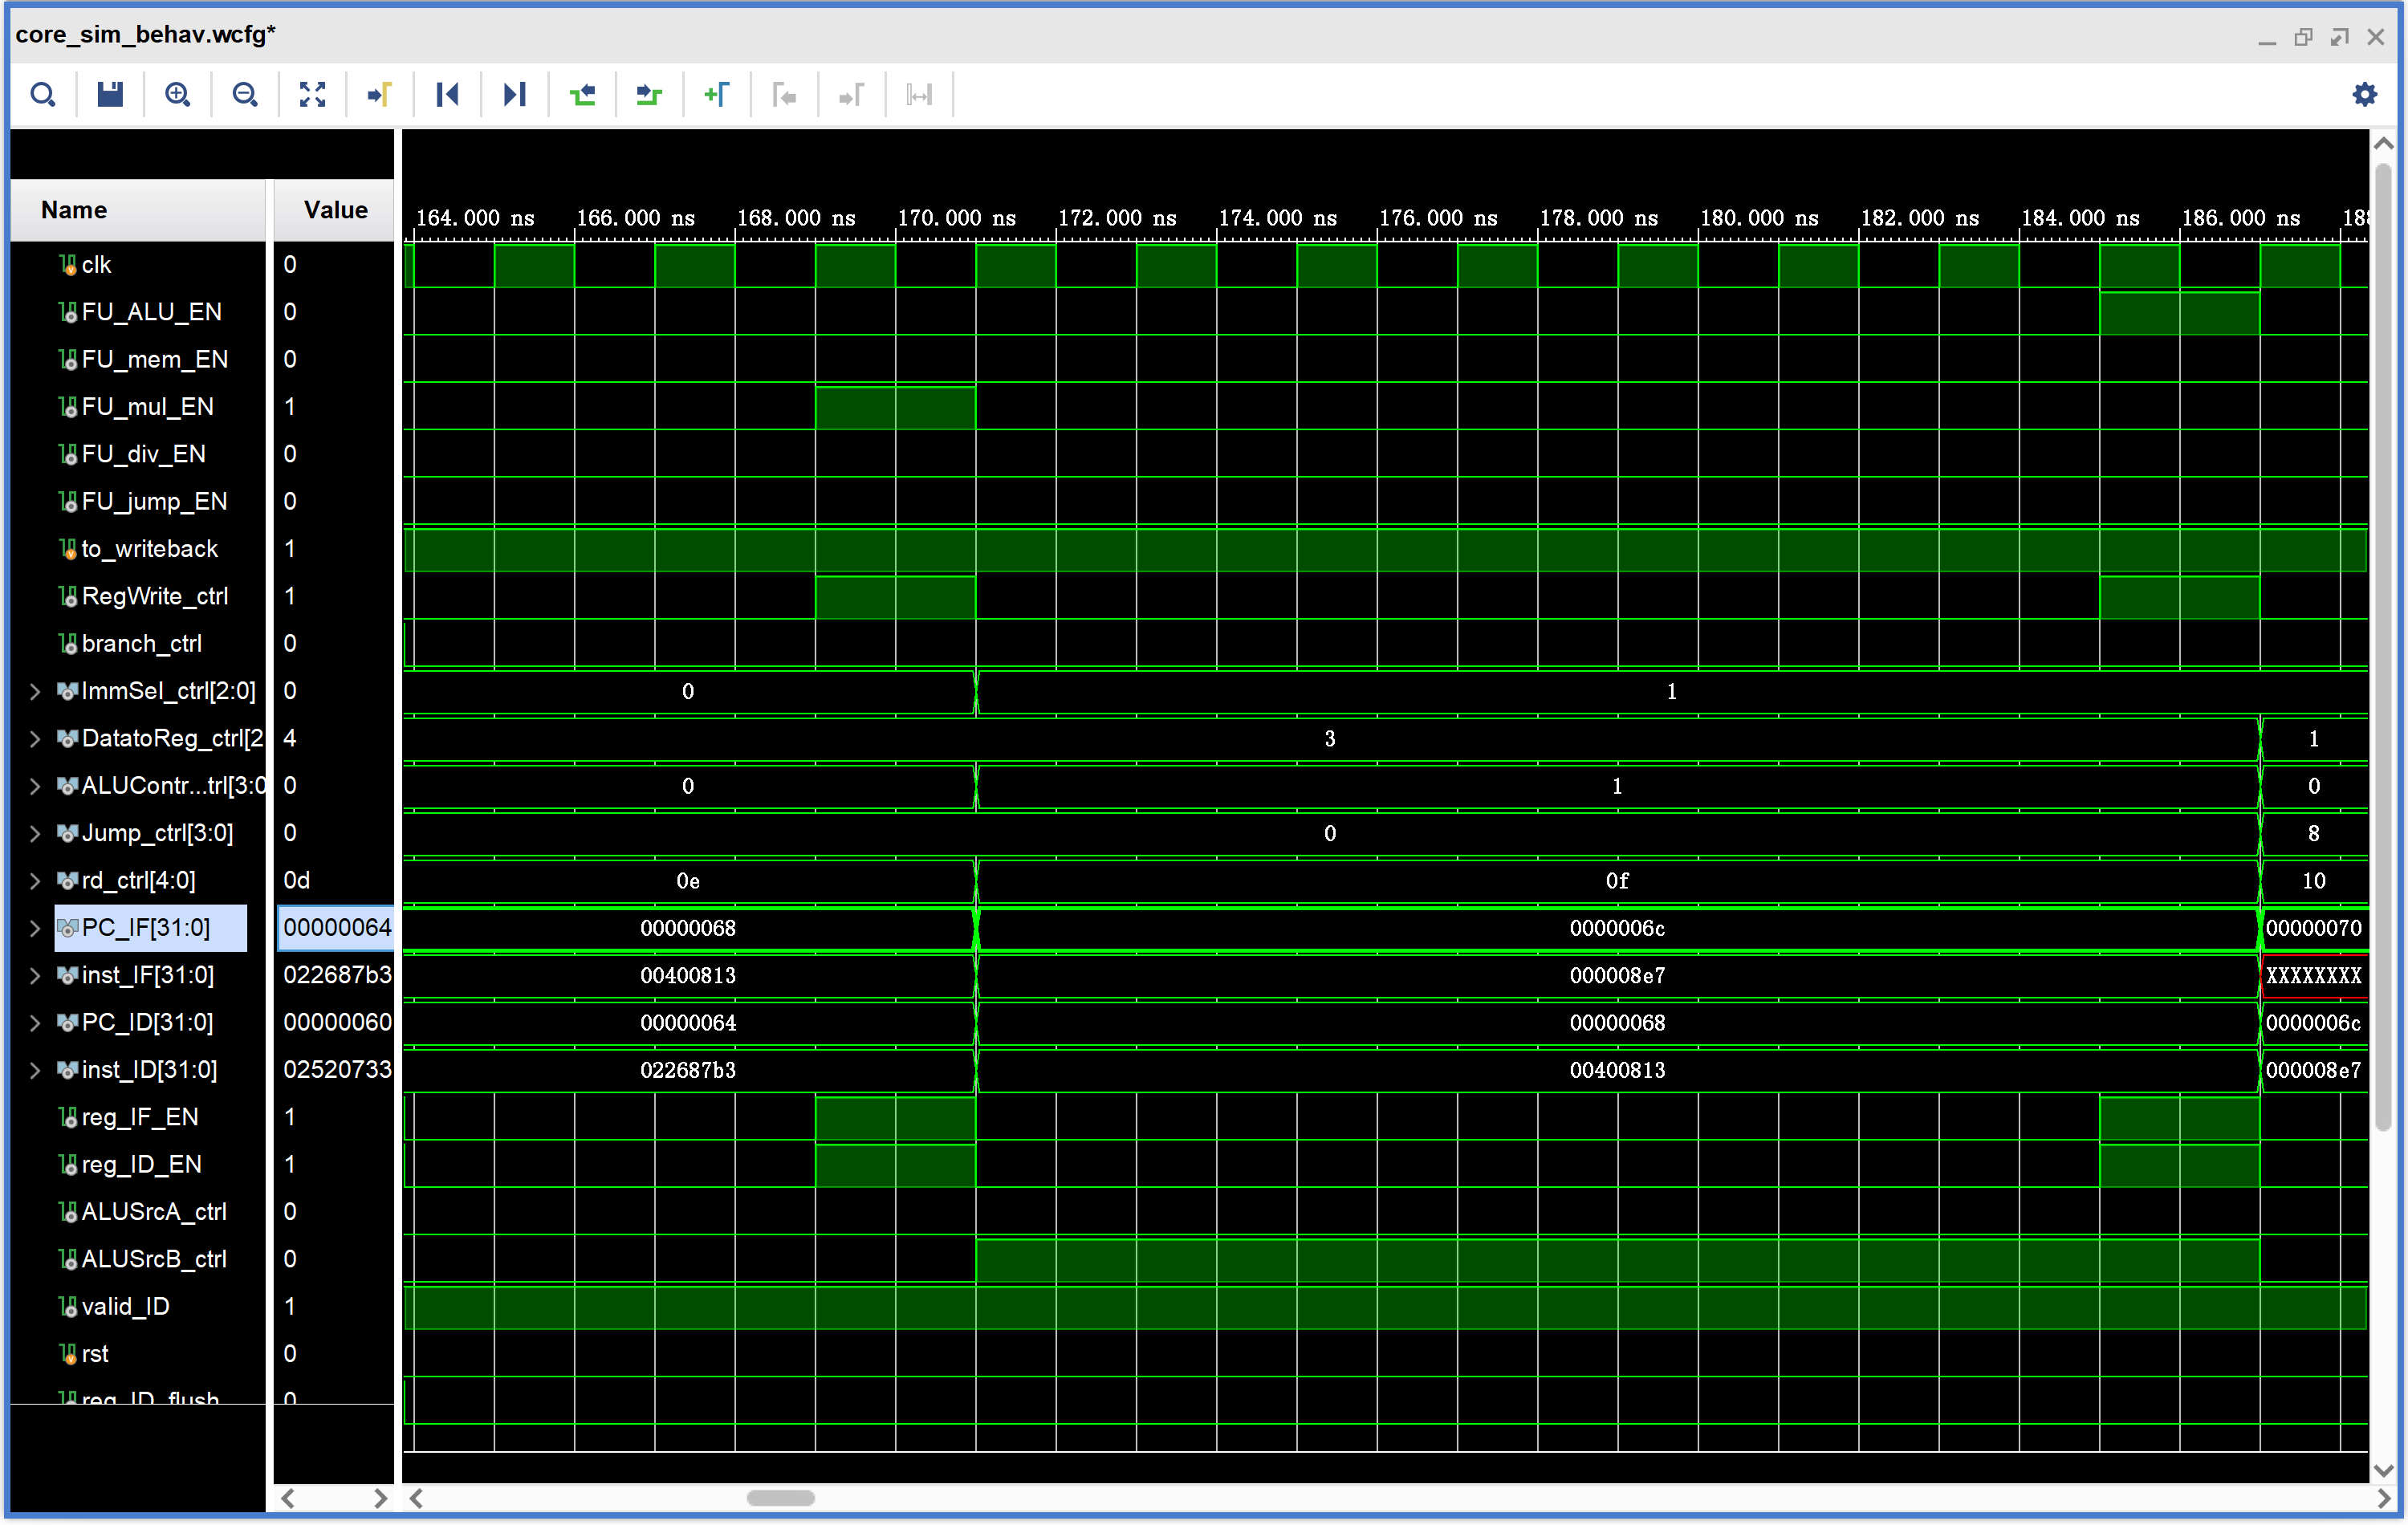
\includegraphics[width=1.0\textwidth]{figs/9.png} %插入图片,[]中设置图片大小,{}中是图片文件名
	\caption{验证结果图3} %最终文档中希望显示的图片标题
	\label{Fig.21} %用于文内引用的标签
\end{figure}
运行至mret后,清空后面的所有指令并跳转回原程序
\begin{figure}[H] %H为当前位置,!htb为忽略美学标准,htbp为浮动图形
	\centering %图片居中
	\includegraphics[width=1.0\textwidth]{figs/10.png} %插入图片,[]中设置图片大小,{}中是图片文件名
	\caption{验证结果图4} %最终文档中希望显示的图片标题
	\label{Fig.22} %用于文内引用的标签
\end{figure}